% Cover letter: PhD R&D Consultant, Aleadin Consulting
% CV: Sections/cv_rd_consultant.tex -> cv_gen/cv_giovanni_tauro-aleadin_consulting.pdf
\documentclass[11pt,a4paper,sans]{moderncv}
% Shared preamble and header for the cover letters.
% One main file per application: cl_<company>.tex, built to
% cv_gen/coverletter_giovanni_tauro-<company>.pdf next to cv_giovanni_tauro-<company>.pdf.
% Paths (cl_gen/..., Pictures/...) are relative to the project root, as in the CV (see .latexmkrc).

\moderncvstyle{classic}
\moderncvcolor{blue}

\usepackage[scale=0.80]{geometry}
\setlength{\footskip}{136.00005pt}

\usepackage{fontawesome5}
% hyperref is loaded by moderncv itself; loading it here causes an option clash
\usepackage{xcolor}
\usepackage{graphicx}
\ifxetexorluatex
  \usepackage{fontspec}
  \usepackage{unicode-math}
  \defaultfontfeatures{Ligatures=TeX}
  \setmainfont{Latin Modern Roman}
  \setsansfont{Latin Modern Sans}
  \setmonofont{Latin Modern Mono}
  \setmathfont{Latin Modern Math}
\else
  \usepackage[T1]{fontenc}
  \usepackage{lmodern}
\fi

\usepackage[english]{babel}

% used for the PDF title and the letter closing; the visible header is \clheader below
\name{Giovanni}{Tauro}

% Header: #1 = headline under the name (same as the headline of the matching CV)
\newcommand{\clheader}[1]{%
\noindent
\begin{minipage}[c]{0.74\textwidth}
    {\Huge \textbf{Giovanni Tauro}}\\[-0.2em]
    {\small #1}\\[0.3em]

    \footnotesize
    \faMapMarker*~
    \href{https://www.google.com/maps/search/?api=1&query=Lecco+23900+Italy}
    {\color{blue}Bari-Lecco, Italy}
    \quad
    \faPhone*~
    \href{https://wa.me/393279437161}
    {\color{blue}+39 3279437161}
    \quad
    \faEnvelope~
    \href{mailto:giovanni.taurodi@gmail.com}
    {\color{blue}giovanni.taurodi@gmail.com}
    \\[-0.1em]

    \faLinkedin~
    \href{https://www.linkedin.com/in/giovanni-tauro-gt/}
    {\color{blue}LinkedIn}
    \quad
    \faGithub~
    \href{https://github.com/jotades}
    {\color{blue}GitHub}
    \quad
    \faGraduationCap~
    \href{https://scholar.google.com/citations?user=BS0aVGgAAAAJ&hl=it}
    {\color{blue}Scholar}
    \quad
    \faFilePdf~
    \href{https://www.notion.so/Giovanni-Tauro-2a7901d92f3a800b892af425c5875c6a}
    {\color{blue}Portfolio}
    \quad
    \faCubes~
    \href{https://grabcad.com/giovanni.tauro-3}
    {\color{blue}GrabCAD}

\end{minipage}
\hfill
\begin{minipage}[c]{0.18\textwidth}
    \raggedleft
    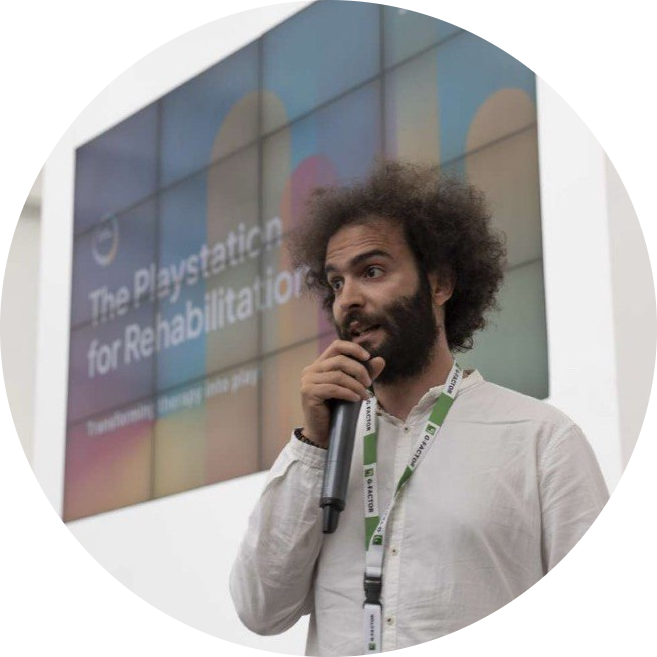
\includegraphics[width=2.8cm]{Pictures/Giovanni_pitch}
\end{minipage}
\vspace{0.1em}
}

\makeatletter
% the sender details are already in \clheader, so skip moderncv's own block
\@detailsfalse
% closing phrase, signature, name
\renewcommand*{\makeletterclosing}{%
  \@closing\\[0.6em]%
  
\includegraphics[height=1.2cm]{Pictures/sign_gt.jpg}\\[0.2em]%
  {\bfseries\@firstname~\@lastname}}
\makeatother


\begin{document}

\clheader{R\&D Engineer, PhD Candidate | Rehabilitation Robotics \& IoT}

\recipient{Recruitment Team}{Aleadin Consulting}
\opening{Dear Hiring Team,}
\closing{Yours faithfully,}
\makelettertitle

I am applying for the PhD R\&D Consultant role. I am an R\&D engineer with more than five years of applied research at CNR-STIIMA, the Italian National Research Council, in rehabilitation robotics, wearable sensing and IoT systems, and I am completing a PhD in Mechanics and Advanced Engineering Sciences at the University of Bologna (expected 2027).

What I can offer your projects is experience in moving research into industry. PhiCube started as a research prototype for bilateral neurorehabilitation. I am co-inventor of its patent (WO2023214349A1) and co-founder and Head of Product of Rehabilia Technologies, the company that develops it as a product. The device was validated with 19 children (SUS 85.8/100) and is now in two ongoing multicentre studies with 134 patients.

On the technical side, my work is experimental design and problem-solving on real systems. For my PhD I designed OmniTrack, an IoT-based multimodal navigation system: I defined its architecture (wearable sensing, indoor localisation, BLE communication, and audio, visual and haptic feedback), built the hardware and software, ran the validation with 16 blind participants and analysed the data in Python. The work is reported in Frontiers in Communications and Networks (2026). Within national programmes such as Fit4MedRob I have also defined requirements with clinicians and delivered prototypes up to deployment in clinics.

A remote, project-based format suits me. I have worked independently during research stays at Utrecht University and Toyo University in Tokyo, I am used to managing my own schedule and deliverables across several projects, and I collaborate daily with engineers, designers and clinicians.

I would be glad to discuss which of your R\&D projects match my profile.

\makeletterclosing

\end{document}
